\section{Tổng quan về BI}
\subsection{Khái niệm}
Kinh doanh thông minh (Business Intelligence - BI) là quy trình/hệ thống công nghệ cho phép phân tích và thể hiện thông tin giúp cho các nhà quản lý và người sử dụng của tổ chức đưa ra các quyết định phù hợp.\\
Kinh doanh thông minh bao gồm một loạt các công cụ, ứng dụng và phương thức cho phép các tổ chức thu thập thông tin từ các hệ thống nội bộ và bên ngoài; chuẩn bị sẵn sàng cho việc phân tích, phát triển và chạy các truy vấn đối với dữ liệu, tạo các báo cáo, bảng điều khiển và hình ảnh hóa dữ liệu để cung cấp kết quả phân tích cho những người sử dụng và những người ra quyết đinh.
\subsection{Các bước trong quy trình kinh doanh thông minh}
\begin{center}
            \begin{figure}[!h]
                \centering
                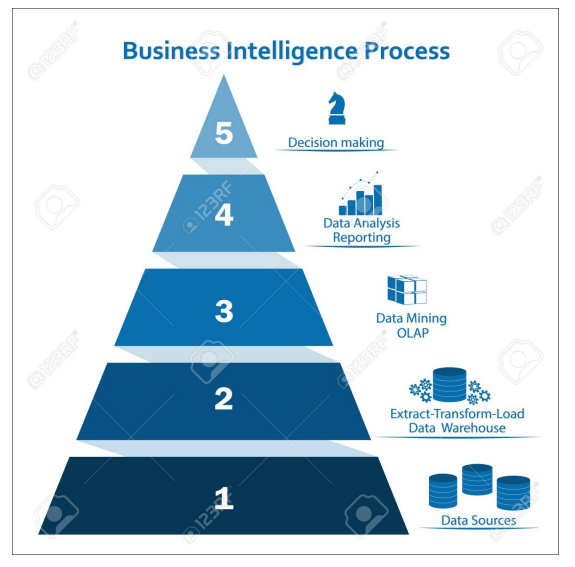
\includegraphics[scale = 1]{figures/Duyen/Quy trình kinh doanh thông minh.PNG}
              \caption{Quy trình kinh doanh thông minh}
            \end{figure}
\end{center}
\newpage
\begin{itemize}[label=$-$]
    \item \textbf{ Nguồn dữ liệu (Data Source)} là vị trí bắt nguồn dữ liệu đang được sử dụng. 
    Nguồn dữ liệu có thể là vị trí ban đầu nơi dữ liệu được sinh ra hoặc nơi thông tin vật lý được số hóa lần đầu tiên, tuy nhiên, ngay cả những dữ liệu tinh tế nhất cũng có thể đóng vai trò là nguồn, miễn là một quy trình khác truy cập và sử dụng nó. Cụ thể, nguồn dữ liệu có thể là một cơ sở dữ liệu đến từ các hệ quản trị cơ sở dữ liệu MySQL, SQL, Oracle, MSSQL, một tệp phẳng, các phép đo trực tiếp từ các thiết bị vật lý, dữ liệu web cóp nhặt hoặc bất kỳ dịch vụ dữ liệu trực tuyến và tĩnh nào có rất nhiều trên internet...
    \item \textbf{Kho dữ liệu (Data Warehouse)} là cơ sở dữ liệu được thiết kế theo mô hình Online Analytical Processing (OLAP), dữ liệu trong data warehouse chỉ có thể đọc, không được ghi hay xóa mà chỉ được update bởi gói ETL chuyển đổi dữ liệu từ Data Sources vào Data Warehouse.
    \item \textbf{Khám phá dữ liệu (Data Exploration)} là bước đầu tiên trong phân tích dữ liệu, trong đó người dùng khám phá một tập dữ liệu lớn theo cách không có cấu trúc để khám phá các mẫu, đặc điểm và điểm quan tâm ban đầu.Khám phá dữ liệu tạo ra các truy vấn, báo cáo, biểu đồ phân tích, thống kê từ mô hình dữ liệu OLAP ở Kho dữ liệu.
    \item \textbf{Khác dữ liệu (Data mining)} là quá trình phân tích khối lượng lớn dữ liệu để khám phá thông tin kinh doanh giúp các công ty giải quyết vấn đề, giảm thiểu rủi ro và nắm bắt cơ hội mới.
\end{itemize}
\subsection{Lợi ích}
Những lợi ích chính mà doanh nghiệp có thể nhận được từ các ứng dụng BI:
\begin{itemize}[label=$-$]
    \item Tăng tốc và cải thiện việc ra quyết định
    \item Tối ưu hóa quy trình kinh doanh nội bộ
    \item Phát hiện các vấn đề kinh doanh cần được giải quyết
    \item Xác định các xu hướng kinh doanh và thị trường mới nổi
    \item Phát triển các chiến lược kinh doanh mạnh mẽ hơn
    \item Thúc đẩy doanh số bán hàng cao hơn và doanh thu mới
    \item Đạt được lợi thế cạnh tranh so với các công ty đối thủ
\end{itemize}
\newpage
Một số công cụ thông dụng hiện nay:
\begin{enumerate}
    \item Power BI
    \item Oracle BI
    \item QlikView
    \item Spago
    \item Pentaho
    \item IBM Cognos
\end{enumerate}
\subsection{ Công cụ trực quan hóa dữ liệu Power BI}
\subsubsection{Giới thiệu chung}
Power BI được ra đời vào năm 2011, được phát triển bởi Microsoft, sau đó nó được đưa vào sử dụng chính thức vào năm 2015. Power BI tập hợp rất nhiều các dịch vụ về phần mềm, các ứng dụng, các trình kết nối hoạt động song song cùng nhau để biến đổi các nguồn dữ liệu từ nhiều nguồn khác nhau thành các thông tin chi tiết liền mạch và trực quan. Power Bi được phát triển, sử dụng trên nền tảng Desktop, Website Service và Mobile App, nó hoàn toàn thân thiện và dễ dàng thích ứng với mọi người dùng mặc dù mỗi người đều có những nhu cầu khác nhau.
\subsubsection{ Các chức năng của Power BI}

\textbf{Kết nối dữ liệu từ nhiều nguồn}\\
Chúng ta có thể truy cập dữ liệu từ nhiều nguồn khác nhau dựa trên nền
tảng Power BI, bao gồm các nguồn như sau:
\begin{itemize}[label=$-$]
    \item File: các dạng Excel, Text/CSV, XML, JSON, Folder, PDF, SharePoint folder.
    \item Database: SQL Server database, Access database, Oracle database, IBM Db2 database, MySQL. . .
    \item Power Platform: Power BI datasets, Power BI dataflows, Common Data Service. . .
    \item Azure
    \item Online Services: SharePoint Online List, Microsoft Exchange Online, Dy-namics 365...
\begin{center}
            \begin{figure}[!h]
                \centering
                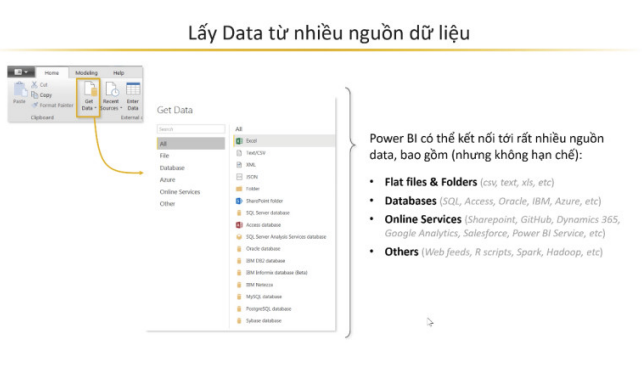
\includegraphics[scale = 1]{figures/Duyen/Kết nối dữ liệu trong PBI.PNG}
              \caption{Kết nối dữ liệu trong PBI}
            \end{figure}
\end{center}
\end{itemize}
\newpage
\textbf{Tiền xử lý dữ liệu}\\
Hầu hết trong doanh nghiệp, dữ liệu thu thập được đều đã trải qua quá trình tiền xử lý dữ liệu để có thể sẵn sàng sử dụng tạo ra các báo cáo. Trong quá trình tiền xử lý dữ liệu, các dữ liệu được trích xuất từ một nguồn dữ liệu, sau đó được chuyển đổi, xác thực, chuẩn hóa, sửa chữa, kiểm tra và cuối cùng được tải vào kho dữ liệu.
\begin{center}
            \begin{figure}[!h]
                \centering
                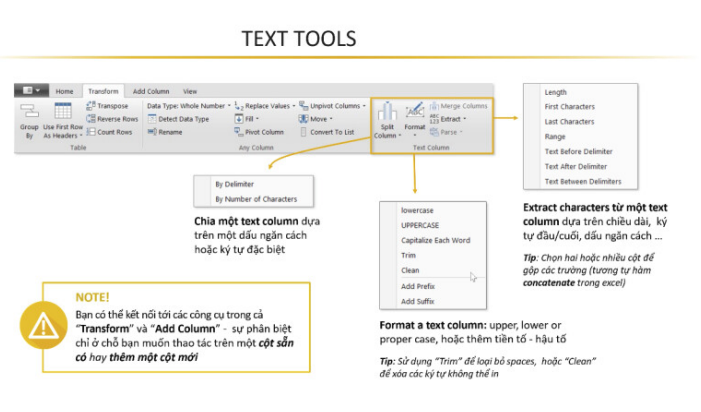
\includegraphics[scale = 1]{figures/Duyen/Tiền xử lý dữ liệu trong PBI.PNG}
              \caption{Kết nối dữ liệu trong PBI}
            \end{figure}
\end{center}
\newpage
Quy trình tiền xử lý dữ liệu được thực hiện bởi các ứng dụng như SQL Server Integration Services (SSIS) hoặc các công cụ của bên thứ ba khác. Tuy nhiên, trong một số doanh nghiệp, công việc tiền xử lý dữ liệu được thực hiện ngay trong Excel, được gọi là chuyển đổi dữ liệu. Tuy nhiên, quy trình ETL trong Excel là một quy trình thủ công, mất nhiều thời gian và khó có thể tự động hóa. \\
Vì thế Microsoft đã tạo ra công cụ để có thể làm cho quá trình này trở nên nhanh và dễ dàng hơn nhiều đó là Power Query, Power BI Desktop. Hai công cụ này cung cấp cho người dùng khả năng tự động hóa quá trình nhập, chuyển đổi và tải dữ liệu vào các bảng nội bộ trong Power BI, sau đó có thể được sử dụng làm nguồn cho các báo cáo hay dashboard của Power BI. Vì Power Query duy trì bản ghi từng bước của mọi hành động được thực hiện để nhập, chuyển đổi và tải dữ liệu, các bước này sẽ được lặp lại khi có thêm dữ liệu được thêm vào.
\textbf{Mô hình hóa dữ liệu (Data modeling)}
Mô hình hóa dữ liệu là quá trình tạo ra một biểu diễn trực quan của toàn bộ hệ thống thông tin hoặc các bộ phận của nó để giao tiếp các kết nối giữa các điểm và cấu trúc dữ liệu. Mục đích là minh họa các loại dữ liệu được sử dụng và lưu trữ trong hệ thống, mối quan hệ giữa các loại dữ liệu này, cách dữ liệu có thể được nhóm và tổ chức cũng như các định dạng và thuộc tính của nó.\\
Dữ liệu có thể được mô hình hóa ở nhiều mức độ trừu tượng khác nhau.
Quá trình bắt đầu bằng cách thu thập thông tin về các yêu cầu kinh doanh từ các bên liên quan và người dùng cuối. Các quy tắc nghiệp vụ này sau đó được chuyển thành cấu trúc dữ liệu để hình thành một thiết kế cơ sở dữ liệu cụ thể.\\
Mô hình dữ liệu có thể được so sánh với lộ trình, bản thiết kế của kiến trúc sư hoặc bất kỳ sơ đồ chính thức nào giúp hiểu sâu hơn về những gì đang được thiết kế.\\
Mô hình hóa dữ liệu sử dụng các lược đồ chuẩn hóa và các kỹ thuật chính
thức. Điều này cung cấp một cách chung, nhất quán và có thể dự đoán được để xác định và quản lý tài nguyên dữ liệu trong một tổ chức hoặc thậm chí xa hơn.\\
Quy trình mô hình hóa dữ liệu:
\begin{itemize}[label=$-$]
    \item Xác định các thực thể
    \item Xác định các thuộc tính chính của từng thực thể
    \item Xác định mối quan hệ giữa các thực thể
    \item Ánh xạ các thuộc tính cho các thực thể hoàn toàn
    \item Gán các khóa khi cần thiết và quyết định mức độ chuẩn hóa cân bằng giữa nhu cầu giảm dư thừa với các yêu cầu về hiệu suất.
    \item Hoàn thiện và xác thực mô hình dữ liệu.
\end{itemize}
\newpage
\textbf{Trực quan hóa dữ liệu}
\begin{center}
            \begin{figure}[!h]
                \centering
                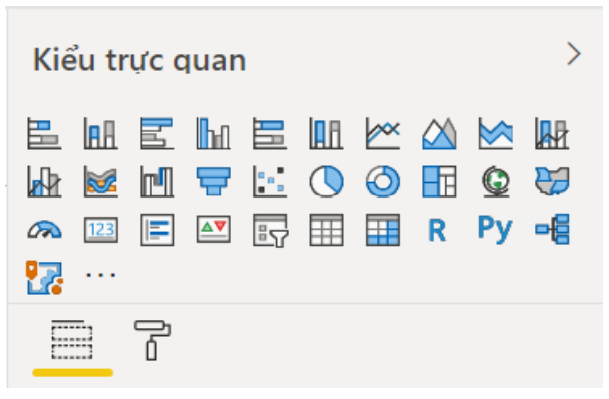
\includegraphics[scale = 1]{figures/Duyen/Các kiểu trực quan hóa dữ liệu trong PBI.PNG}
              \caption{Kết nối dữ liệu trong PBI}
            \end{figure}
\end{center}
Trực quan hóa dữ liệu là biểu diễn đồ họa của thông tin và dữ liệu. Bằng cách sử dụng các yếu tố trực quan như biểu đồ, đồ thị và bản đồ, các công cụ trực quan hóa dữ liệu cung cấp một cách dễ tiếp cận để xem và hiểu các xu hướng, ngoại lệ và mẫu trong dữ liệu.\\
Trong thế giới của Dữ liệu lớn, các công cụ và công nghệ trực quan hóa dữ liệu là rất cần thiết để phân tích một lượng lớn thông tin và đưa ra các quyết định dựa trên dữ liệu.\\
Trực quan hóa dữ liệu giúp bạn biến tất cả dữ liệu chi tiết đó thành thông tin kinh doanh dễ hiểu, hấp dẫn về mặt hình ảnh — và hữu ích.\\
Trực quan hóa dữ liệu làm cho dữ liệu trở nên sống động, khiến bạn trở thành người kể chuyện bậc thầy về những thông tin chi tiết ẩn trong các con số của bạn. Thông qua trang tổng quan trực tiếp, báo cáo tương tác, biểu đồ, đồ thị và các biểu thị trực quan khác, trực quan hóa dữ liệu giúp người dùng phát triển thông tin chi tiết mạnh mẽ về doanh nghiệp một cách nhanh chóng và hiệu quả.




